\chapter{Génération automatique de texte}

Ce sera une section du mémoire sur le mécanisme dsynt=X

\section{Mécanisme dsynt=created->constrained->OK pour générer un énoncé simple (sujet, verbe, objet)}

\subsection{application de la règle root{\_}standard}
Cette règle crée un noeud qui sera la racine de l'arbre syntaxique. Ce noeud se fait imposer des contraintes. Notamment, on demande à ce que ce soit un lexème appartenant à la partie du discours : verbe et que sa finitude soit de type: fini. On impose à ce noeud le trait dsynt=constrained pour que ça s'harmonise avec le règle lex{\_}standard, mais c'est à revoir.

\subsection{application de la règle lex{\_}standard pour lexicaliser le verbe principal}
On assigne un lexème à un noeud  créé en syntaxe profonde. Dans le contexte actuel, on l'utilise pour sélectionner l'unité lexicale qui matche les contraintes énoncées sur le noeud vide créé par la règle root{\_}standard. Ce lexème provient du lexicon.Lorsque la règle s'applique et qu'elle consomme le noeud en y mettant la bonne lexicalisation (qui respecte les contraintes sur le noeud), on ajoute un trait dsynt=OK pour signifier que le sémantème a été réalisé en syntaxe profonde et qu'on ne fasse plus d'opérations sur ce noeud.

\subsection{application de la règle actant{\_}gp{\_}selection}
Cette règle s'applique lorsque nous avons un prédicat.
On crée une variable[ ?GP] qui nous fournit un chemin vers l'information encodée sous l'attribut \emph{ gp} d'un lexème [?X]. Puis , on extirpe les traits \emph{ id} et \emph{dia} pour chaque attribut\emph{ gp} de notre [?X]. Une fois qu'on a récupéré ces informations, on les appose au lexème en question car on se servira de ces informations pour l'application de règles subséquentes. Le trait \emph{ id} représente la description du patron de régime (chaque description se retrouve dans notre gpcon qui est un dictionnaire de\emph{ gp}) et le trait dia nous renseigne sur la diathèse de ce patron de régime, c'est-à-dire combien d'actants sont en jeu, et dans quel ordre sont-ils placés ? Il est essentiel qu'un lexème verbal aille chercher ces traits car il en a besoin pour appliquer les règles actancielles qui en découlent. Il faut que le système sache quel patron de régime utilisé pour un prédicat donné, et dans quel ordre les actants seront réalisés en syntaxe.

\subsection{application des règles actancielles}
Une fois qu'un gp est sélectionné, on appliquera la règle actancielle qui lui correspond. Nos règles actancielles ressemblent à : actant{\_}gp{\_}ijk. Les règles prennent en input les arcs sémantiques liant les actants à leur prédicat. Ces règles génèrent des noeuds vides auxquels on appose un trait dsynt=created pour signifier qu'on vient de créer des noeuds vides (on dit qu'ils sont vides car ils n'ont pas encore été consommés par une unité lexicale) en syntaxe profonde. On obtient ainsi des arcs syntaxiques au bout desquels se trouve un noeud vide. Ces règles se font imposer des conditions bien strictes. Il faut d'abord que le prédicat qui les gouverne soit lexicalisé. Ce qui se traduisait par l'ajout d'un trait dsynt=OK au lexème lexicalisé (avec la règle lex{\_}tandard). La règle actant{\_}gp{\_}selection nous permettait de soutirer les traits  \emph{ id} et \emph{dia} et c'est ici que le trait dia entre en jeu. On s'en sert pour illustrer la diathèse du verbe. [à revoir]

\subsection{application de la règle constraints{\_}gp}
Cette règle applique des contraintes à des noeuds nouvellement créés (autrement dit, des noeuds qui ont le trait dsynt=created). C'est à partir de cette règle que le mécanisme de \emph{dsynt=created-> constrained->OK} prend vie. Il s'agit d'une étape intermédiaire entre la création du noeud avec les règles actancielles et la lexicalisation qui consommera le noeud en octroyant un lexème suivant un trait dsynt=OK (signifiant que la réalisation en syntaxe profonde est terminée). Ainsi, la règle procède de cette manière. On prend un X (un prédicat) qui lie un Y (un actant) puis ce dernier se fait imposer des contraintes. On cherche à lui imposer ces contraintes car on souhaite qu'il respecte le patron de régime de X. Ainsi, s'il ne convient pas comme actant syntaxique, il ne pourra pas passer à la lexicalisation. Car on souhaite une correspondance entre les traits naturels contenus dans le dictionnaire pour le sémantème en question. Si ses traits ne convienne pas aux contraintes imposées au noeud, provenant du patron de régime de X, alors l'arbre sera incomplet. Lorsqu'on met les contraintes sur le noeud, on lui met aussi le trait dsynt=constrained pour montrer qu'il a été contraint et donc qu'il remplit les critères pour passer à la lexicalisation.

\subsection{application des règles de lexicalisation}

Il y a différentes règles de lexicalisation afin de donner un peu de latitude au système. Ainsi, si quelques informations sont manquantes dans le lexicon ou le semanticon, nous voulons que le système arrive quand même à effectuer une génération de texte. C'est pourquoi il existe la règle standard qui fonctionne lorsque nous avons accès à tous les éléments nécessaires. Les régles de types \emph{guess} opèrent lorsqu'il nous manque certaines infos. 

\subsubsection{lex{\_}standard}

Nous avons vu cette règle un peu plus haut, car il fallait l'appliquer dès le début pour lexicaliser le noyau principal afin de chercher le bon lexème qui pouvait remplir cette fonction. Une fois que nous l'avons lexicalisé, nous avons pu aller chercher les informations sur la nature de son gp etc. Nous sommes maintenant rendus au moment où il existe des arcs syntaxiques au bout desquels nous avons des noeuds contraints par des traits comme : la dpos, la finitude, la définitude, etc. Nous allons donc lexicaliser ces noeuds afin de poursuivre la construction de l'arbre, du haut vers le bas. En gros, comment ça fonctionne. On cherche la lexicalisation d'un sémantème donné dans le semanticon, en allant chercher le trait \emph{lex} du sémantème. Puis, on colle cette lexicalisation a un noeud déjà existant. Ce noeud existe déjà car il a soit été créé par root{\_}standard ou par une des règles actancielles. On va octroyer au noeud 3 traits : un trait dlex, un trait dpos, et finalement un trait dsynt. Le trait dlex est la lexicalisation profonde, celle qu'on retrouve dans le lexicon, le trait dpos est la partie du discours profonde qui doit correspondre à la dpos demandée par constraints{\_}gp. Et finalement, un trait dsynt=OK qui s'ajoute à la lexicalisation du sémantème pour signifier au système que le noeud a été consommé et qu'il a été réalisé en syntaxe profonde. Donc, qu'on ne fasse plus d'opération sur ce noeud. Finalement, on peut uniquement faire des opérations sur des noeuds qui ont let trait dsynt=constrained afin de lexicaliser seulement les noeuds qui se sont fait attribués des contraintes. Ainsi, s'ils respectent les contraintes, ils pourront être lexicalisé, sinon, l'arbre sera incomplet et la génération échouera.

\subsection{Avantages d'utiliser ces mécanismes}

"Dsynt=OK" indique que le noeud a été consommé. Autrement dit, il existe maintenant une unité lexicale réalisé en syntaxe profonde, là où il y avait un noeud vide.
"Dsynt=constrained" indique qu'un noeud vide s'est fait imposé des contraintes. Ces contraintes peuvent être de plusieurs ordres. Notamment, on impose une dpos, une finitude, un mood, etc. Il s'agit du passsage intermédiaire entre la création d'un noeud et sa lexicalisation. On veut s'assurer qu'il respecte certaines contraintes pour ne pas lexicaliser n'importe quoi lors de la génération de notre arbre syntaxique.
Finalement, le trait dsynt=created 

\section{Énumérations}

Voici une énumération avec numérotation :
\begin{enumerate}
	\item item 1;
	\item item 2;
	\item item 3.
\end{enumerate}
Maintenant, une énumération sans numérotation avec des marqueurs différents :
\begin{itemize}
	\item Marqueur par défaut;
	\item[$\bullet$] \verb|$\bullet$|;
	\item[$\star$] \verb|$\star$|.
\end{itemize}


\section{Équations mathématiques}

Une équation :
\begin{equation*}
	\otimes^n\,\mathbb{C}^2 \cong \bigoplus_{m=-n/2}^{n/2} W_m.
\end{equation*}

Une autre équation, cette fois-ci numérotée :
\begin{equation}
	\label{eq:eulerlagrange}
	\frac{\partial\mathcal{L}}{\partial\phi^a}-\partial_\mu\frac{\partial\mathcal{L}}{\partial(\partial_\mu\phi^a)}=0,\qquad\mu=0,1,2,3.
\end{equation}
Les équations \eqref{eq:eulerlagrange} précédentes sont appelées \emph{équations d'Euler-Lagrange} ou encore \emph{équations du mouvement}. Dans les calculs suivants,
\begin{align*}
	\delta S	& = \int_\Omega\mathrm{d}^dx\,\mathcal{L}\bigl(\phi'^a(x),\partial_\mu\phi'^a(x)\bigr)-\int_\Omega\mathrm{d}^dx\,\mathcal{L}\bigl(\phi^a(x),\partial_\mu\phi^a(x)\bigr)																												\\
				& = \int_\Omega\mathrm{d}^dx\,\left[\delta\phi^a\frac{\partial\mathcal{L}}{\partial\phi^a}+\partial_\mu\delta\phi^a\frac{\partial\mathcal{L}}{\partial(\partial_\mu\phi^a)}\right]																									\\
				& = \int_\Omega\mathrm{d}^dx\,\left[(\delta\phi^a\frac{\partial\mathcal{L}}{\partial\phi^a}+\partial_\mu\left(\delta\phi^a\frac{\partial\mathcal{L}}{\partial(\partial_\mu\phi^a)}\right)-\delta\phi^a\partial_\mu\frac{\partial\mathcal{L}}{\partial(\partial_\mu\phi^a)}\right]	\\
				& = 0,
\end{align*}
aucune ligne n'est numérotée. Alors que dans ce qui suit, la derni\`ere ligne l'est :
\begin{align}
	\delta S	& = \int_{\Omega'}\mathrm{d}^dx'\,\mathcal{L}\bigl(\phi'^a(x'),\partial'_\mu\phi'^a(x')\bigr)-\int_\Omega\mathrm{d}^dx\,\mathcal{L}\bigl(\phi^a(x),\partial_\mu\phi^a(x)\bigr)																															\notag\\
				& = \int_\Omega\mathrm{d}^dx\,\left[\bar{\delta}\phi^a\frac{\partial\mathcal{L}}{\partial\phi^a}+\partial_\mu\bar{\delta}\phi^a\frac{\partial\mathcal{L}}{\partial(\partial_\mu\phi^a)}\right]+\int_{\partial\Omega}\mathrm{d}\sigma_\mu\,\mathcal{L}\bigl(\phi^a,\partial_\mu\phi^a\bigr)\delta x^\mu	\notag\\
				& = \int_\Omega\mathrm{d}^dx\,\partial_\mu\mathcal{J}^\mu(x).	\label{eq:variationaction}
\end{align}


\section{Définitions, théor\`emes et preuves}

Voici une définition.
\begin{deff}[La définition]
	La définition.
\end{deff}
Voici un théor\`eme.
\begin{theo}[Titre]
	Ceci est vrai !
\end{theo}
\begin{proof}
	Voici la preuve.
\end{proof}
\begin{demo}
	Voici la preuve en gras.
\end{demo}


\section{Construction d'un tableau}

\begin{table}[htb]
	\centering
	\caption{Un tableau simple dans le second chapitre.}
	\label{tab:simple2}
	\begin{tabular}{|c||l|c|r|p{0.4\textwidth}|}
		\hline			&			&			&			&																															\\
		\textbf{Option}	& g			& c			& d			& \verb|p{0.4\textwidth}|																									\\[3mm]
		\hline\hline	&			&			&			&																															\\
		\textbf{Effet}	& À gauche	& Au centre	& À droite	& Le texte de cette colonne est justifié et la largeur de la colonne est fixée \`a 40\,\% de la zone de texte (hors tableau).	\\[3mm]
		\hline 
	\end{tabular}
\end{table}
Le tableau \ref{tab:simple2} n'est pas tr\`es garni.

\section{Référence \`a une entrée bibliographique}

Les documents par \citet{Lamport1986,GMS1994} ainsi que \citet{Spivak1990} 
sont des références en mati\`ere de \LaTeX. Le manuel par 
\citet{GMS1994} est probablement le plus populaire du lot.

L'article de \citet{Martin1992} est, manifestement, tr\`es riche en rebondissements.

Les entrées du fichier \verb|.bib| qui ne sont pas référencées 
dans le texte ne sont pas ajoutées \`a la bibliographie : un avantage 
de plus en faveur de Bib\TeX.

Dans ce paragraphe, on teste une cette référence \citet{hastie2005}.

\section{Insertion de figures}

% Voici deux types d'insertion de figures.

\begin{figure}[t]
	\centering
	
\includegraphics[width=0.2\textwidth]{ch3/figs/cercle.pdf}
	\caption{Un cercle.}
	\label{fig:Cercle}
\end{figure}

La figure \ref{fig:Cercle} est un \emph{cercle}.
\begin{figure}[t]
	\centering
	\subfigure[Un triangle.]{\label{fig:Triangle}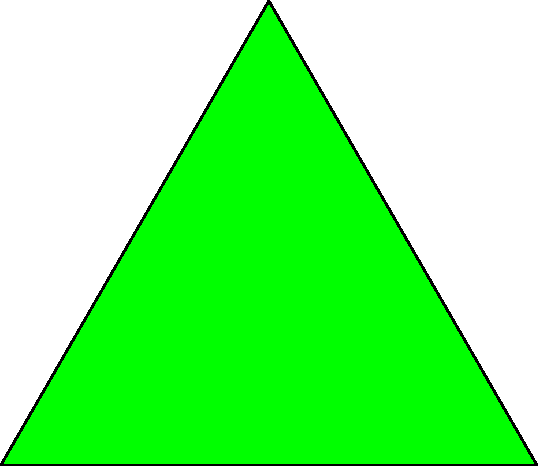
\includegraphics[width=0.2\textwidth]{ch3/figs/triangle.pdf}}\hspace{2cm}
	\subfigure[Un carré.]{\label{fig:Carre}
\includegraphics[width=0.2\textwidth]{ch3/figs/carre.pdf}}
	\caption{\label{fig:TriCar}Un carré et un triangle.}
\end{figure}
À la figure \ref{fig:TriCar}, le triangle \subref{fig:Triangle} et le carré \subref{fig:Carre} ont été placés côtes-\`a-côtes grâce \`a la commande \verb|\subfigure|. 



